\section{Teori}

\subsection{Raspberry Pi}
Raspberry Pi er datamaskinen i dette prosjektet. Det ble valgt for å bruke RPi fordi det er en kraftig datamaskin som kan kjøre programmer raskt, samtidig som den har GPIO-pinner som gir mulighet for tilkobling av ekstern tilkobling. RPi-en kan også kobles til GitHub, noe som gir en raskere og enklere arbeidsflyt. I tillegg støtter RPi-en alle kommunikasjonsprotokollene vi trengte i prosjektet, blant annet I2C og bit bang.

\subsection{PCA9685}
For å kunne kontrollere flere servomotorer samtidig ved bruk av RPi-en, brukte man chippen PCA9685. Denne gjør det mulig å styre opptil 16 servomotorer via I2C, med presise og stabile PWM signaler enn hva RPi-en kan gi.

\subsubsection{I2C}
I2C er kommunikasjon protokollen som blir brukt i PCA9685. I2C blir vanligvis brukt å koble mellom mikrokontrollere og sensorer, minnebrikker og andre enheter. 

Buss strukturen til I2C er en synkron toveis kommunikasjonsbuss som kun benytter av to ledere: SDA (Serial Data) som er linjen som overfører data og SCL (Serial Clock) som er klokken som synkroniserer dataoverføringen laget av master enheten.

Kommunikasjonen bruker master og slave prinspit. Det er en master enhet (vanligvis en mikrokontoler eller RPi i dette prosjektet) som styrer klokkesignalet og initialerer komunaksjonen. Og slave enheter svarer når kun de er addresert. Man kan tenke seg slikk at master enheten er posten som levere ut inviasjonen og slaven kan bare svare hvis de har fått invitasjoner. Hver slave har en unik addresse som er regel på 7 bit. Det gir i teori opp til 128 enheter på samme buss linje.

\colorbox{yellow}{placeholder}
Data overføring skjer slik ut. 
Masteren sender en startbetingelse (SDA går lav mens SCL er høy).
Masteren sender slavens 7-bits adresse fulgt av en lese-/skrivebit (R/ som angir overføringsretning.
Den adresserte slaven svarer med et ACK-bit (acknowledge) for å bekrefte at den er tilstede.
Data overføres byte for byte, hvor hver byte etterfølges av et ACK- eller NACK-bit fra mottakeren.
Masteren avslutter med en stoppbetingelse (SDA går høy mens SCL er høy).

\subsection{HX711}
For å måle vekten på glassene brukte vi chippen HX711. Denne chippen leser av analoge signaler fra en lastcelle og konverterer dem til digitale data. HX711 er en 24 bits analog til digital omformer (ADC) spesielt beregnet for lastceller. Chippen kommuniserer med RPi-en via sin egen serielle protokoll basert på bit-banging. Siden hver HX711 kun kan lese fra en lastcelle, måtte vi ta i bruk tre chipper for å kunne lese av tre lastceller.

\subsubsection{Bit bang}

\subsection{Dual H-Brigde L298N module}
Modulen bruker både 5V og 12V. Den mottar et PWM-signal og har i tillegg en «HIGH-pin» og en «LOW-pin» som bestemmer hvilken retning pumpen går. Bytter man om på disse to pinnene, snur pumpe retningen.

Modulen er en dobbel bidireksjonell H-bro. Det betyr at den kan styre to DC-motorer samtidig uavhengig av hverandre. En H-bro er en standard-krets av fire transistorer satt sammen i en form som ligner på bokstaven H, hvor motoren er plassert i midten. Med å aktivere diagonalt motsatte transistorer kan strømmen gå gjennom motoren, og å aktivere motsatte transistorer vil de gå motsatt vei.

PWM-signalet brukes til å styre hastigheten på motoren. PWM-en veksler raskt mellom «HIGH» og «LOW», og forholdet mellom "HIGH" tid og "LOW" tid kalles «duty cycle». En høy duty cycle gir motoren høyere hastighet, mens en lav duty cycle gir lavere hastighet.

\subsection{Regulering}
For å fylle glasset og sikre at det blir fylt opp uten søl, brukes en form for regulering. En regulator sin oppgave er å styre et system slik at den målte $y(t)$ følger en ønsket referanseverdi så presist som mulig. I dette prosjektet styres pumpen ut fra hvor mye væske som skal være i glasset, slik at fyllingen stoppes på riktig tidspunkt.

\begin{figure}[H]
    \centering
    \includesvg[width=1\linewidth]{Images/PID.svg}
    \caption{PID sløyfe}
    \label{fig:PID_diagram}
\end{figure}

Reguleringen er bygget opp som en \emph{lukket sløyfe}. Det innebærer at den målte $y(t)$ kontinuerlig sammenlignes med referanseverdien, og at differansen mellom dem brukes til å bestemme pådraget. Feilsignalet er definert som differansen mellom referanseverdien $y_0(t)$ og målte ut verdien $y(t)$:
\begin{equation}
    e(t) = y_0(t) - y(t)
\end{equation}

Uten PID følger kontrolleren en på/av-logikk:
\begin{equation}
    u(t) = \begin{cases} 1 & \text{hvis } e(t) > 0 \\ 0 & \text{hvis } e(t) \leq 0 \end{cases}
\end{equation}

For å oppnå en jevnere og mer presis styring brukes en PID regulator. PID regulatoren består av: et proporsjonalt ledd (P), et integrasjoins ledd (I) og et deriverende ledd (D). 

Og under er $K_p$, $K_i$ og $K_d$ forsterkningskonstantene for henholdsvis proporsjonal, integral og derivasjons leddet. Disse må tunes inn for å gi ønsket oppførsel, der målet er en rask respons med lite oversving og liten stasjonær feil og unngå oscillasjon.
\begin{equation}
    u(t) = K_p \cdot e(t) + K_i \int_0^t e(\tau)\,d\tau + K_d \frac{de(t)}{dt}
\end{equation}

Den diskrete formelen som brukes i koden er:
\begin{equation}
    u[k] = K_p \cdot e[k] + K_i \sum_{j=0}^{k} e[j] \cdot \Delta t + K_d \frac{e[k]-e[k-1]}{\Delta t}
\end{equation}

Integralleddet er her tilnærmet med en Riemann sum, der feilen i hvert tidssteg multipliseres med $\Delta t$ og summeres opp. Derivasjonsleddet er tilnærmet med baklengs differanse (finite difference), altså endringen i feilsignalet fra forrige til nåværende tidssteg delt på $\Delta t$. Disse tilnærmingene blir mer nøyaktige jo mindre $\Delta t$ er.

\subsection{Invers kinematikk}
For å styre bevegelsen til robotarmen brukte vi en forenklet versjon av invers kinematikk. Vi valgte invers kinematikk fremfor fremoverkinematikk fordi fremoverkinematikk beregner endepunktet ut fra kjente leddvinkler, mens invers kinematikk gjør det motsatte den beregner nødvendige leddvinkler for å oppnå en ønsket endeposisjon. Robotarmens geometri er illustrert i figur \ref{fig:3dof}.

\begin{figure}[H]
    \centering
    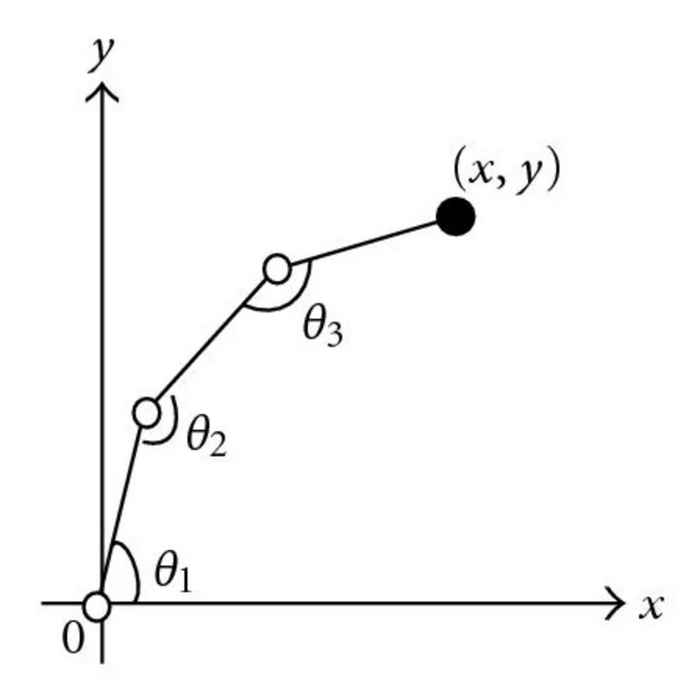
\includegraphics[width=0.5\linewidth]{Images/Placeholder_3dof_grafh.png}
    \caption{Diagram over robotarmens geometri med tre frihetsgrader.}
    \label{fig:3dof}
\end{figure}

Vi definerer håndleddspunktet $(x_w, y_w)$ ved å trekke fra bidraget fra det siste leddet med lengde $L_3$:
\begin{align}
    x_w &= x - L_3 \cos(\varphi) \\
    y_w &= y - L_3 \sin(\varphi)
\end{align}
Vinkelen $\theta_2$ finnes ved hjelp av cosinussetningen:
\begin{align}
    \cos(\theta_2) &= \frac{x_w^2 + y_w^2 - L_1^2 - L_2^2}{2 L_1 L_2} \\
    \theta_2 &= \text{atan2}\!\left(\pm\sqrt{1 - \cos^2(\theta_2)},\ \cos(\theta_2)\right)
\end{align}
Deretter beregnes $\theta_1$ og $\theta_3$:
\begin{align}
    \theta_1 &= \text{atan2}(y_w,\ x_w) - \text{atan2}(L_2 \sin(\theta_2),\ L_1 + L_2 \cos(\theta_2)) \\
    \theta_3 &= \varphi - \theta_1 - \theta_2
\end{align}